\documentclass[]{article}
\usepackage{lmodern}
\usepackage{amssymb,amsmath}
\usepackage{ifxetex,ifluatex}
\usepackage{fixltx2e} % provides \textsubscript
\ifnum 0\ifxetex 1\fi\ifluatex 1\fi=0 % if pdftex
  \usepackage[T1]{fontenc}
  \usepackage[utf8]{inputenc}
\else % if luatex or xelatex
  \ifxetex
    \usepackage{mathspec}
  \else
    \usepackage{fontspec}
  \fi
  \defaultfontfeatures{Ligatures=TeX,Scale=MatchLowercase}
\fi
% use upquote if available, for straight quotes in verbatim environments
\IfFileExists{upquote.sty}{\usepackage{upquote}}{}
% use microtype if available
\IfFileExists{microtype.sty}{%
\usepackage{microtype}
\UseMicrotypeSet[protrusion]{basicmath} % disable protrusion for tt fonts
}{}
\usepackage[margin=1in]{geometry}
\usepackage[unicode=true]{hyperref}
\hypersetup{
            pdftitle={methodological \& statistical issues to communicate in research proposals},
            pdfauthor={w.cools (ICDS)},
            pdfborder={0 0 0},
            breaklinks=true}
\urlstyle{same}  % don't use monospace font for urls
\usepackage{graphicx,grffile}
\makeatletter
\def\maxwidth{\ifdim\Gin@nat@width>\linewidth\linewidth\else\Gin@nat@width\fi}
\def\maxheight{\ifdim\Gin@nat@height>\textheight\textheight\else\Gin@nat@height\fi}
\makeatother
% Scale images if necessary, so that they will not overflow the page
% margins by default, and it is still possible to overwrite the defaults
% using explicit options in \includegraphics[width, height, ...]{}
\setkeys{Gin}{width=\maxwidth,height=\maxheight,keepaspectratio}
\IfFileExists{parskip.sty}{%
\usepackage{parskip}
}{% else
\setlength{\parindent}{0pt}
\setlength{\parskip}{6pt plus 2pt minus 1pt}
}
\setlength{\emergencystretch}{3em}  % prevent overfull lines
\providecommand{\tightlist}{%
  \setlength{\itemsep}{0pt}\setlength{\parskip}{0pt}}
\setcounter{secnumdepth}{0}
% Redefines (sub)paragraphs to behave more like sections
\ifx\paragraph\undefined\else
\let\oldparagraph\paragraph
\renewcommand{\paragraph}[1]{\oldparagraph{#1}\mbox{}}
\fi
\ifx\subparagraph\undefined\else
\let\oldsubparagraph\subparagraph
\renewcommand{\subparagraph}[1]{\oldsubparagraph{#1}\mbox{}}
\fi
\usepackage{titling}
\usepackage[export]{adjustbox}
\pretitle{%
  \begin{center}
  \LARGE
  \begin{figure}[!h]
  	\begin{minipage}{4cm}
  		
\includegraphics[width=4cm,height=1cm,left]{icds.png}\\[\bigskipamount]
  	\end{minipage}
  	\hfill
  	\begin{minipage}{4cm}	
  		
\includegraphics[width=4cm,height=1cm,right]{umc.png}\\[\bigskipamount]
  	\end{minipage}
  \end{figure}
}
\posttitle{\end{center}
}

\title{methodological \& statistical issues\\
to communicate in research proposals}
\author{w.cools (ICDS)}
\date{\today}

\begin{document}
\maketitle

Current draft aims to introduce researchers to the key ideas in research
methodology that would help them plan their study and write a research
proposal. Our target audience is primarily the research community at VUB
/ UZ Brussel, those applying for funding at the WFWG in particular.\\
\\
Note that we present our view, suitable for communicating research at
VUB / UZ Brussel, not necessarily outside. Therefore, what we present
should only be used for guidance, not as an argument or proof of any
kind.\\
\\
We invite you to help us improve this document by sending us feedback
\href{mailto:wilfried.cools@vub.be}{\nolinkurl{wilfried.cools@vub.be}}
or anonymously at www.icds.be/consulting (right side, bottom)

\newpage

\section{Methodology and Statistics: Research
Proposal}\label{methodology-and-statistics-research-proposal}

\begin{itemize}
\tightlist
\item
  convince referees that

  \begin{itemize}
  \tightlist
  \item
    your study can provide an interesting contribution to your field of
    research
  \item
    your study will be successful: effective and efficient
  \item
    your findings will outweigh the cost

    \begin{itemize}
    \tightlist
    \item
      to apply for funding: show return value of investment, for example
      scientific merit
    \item
      to apply for ethical approval: show necessity of all potential
      risk/harm/stress/\ldots{} \\
    \end{itemize}
  \end{itemize}
\item
  beware: some referees are statisticians who do not understand your
  area of expertise

  \begin{itemize}
  \tightlist
  \item
    include necessary methodological / statistical components
  \item
    in a way a statistical referee understands
  \end{itemize}
\end{itemize}

\section{Key Ingredients}\label{key-ingredients}

\begin{itemize}
\tightlist
\item
  aim of the study: what you want (confirmatory, exploratory,
  preparatory, techn(olog)ical)
\item
  design of the study: how you can do it (quantity, quality,
  generalization)
\item
  aim should match design: often linked by statistics 
\end{itemize}

\begin{figure}[htbp]
\centering
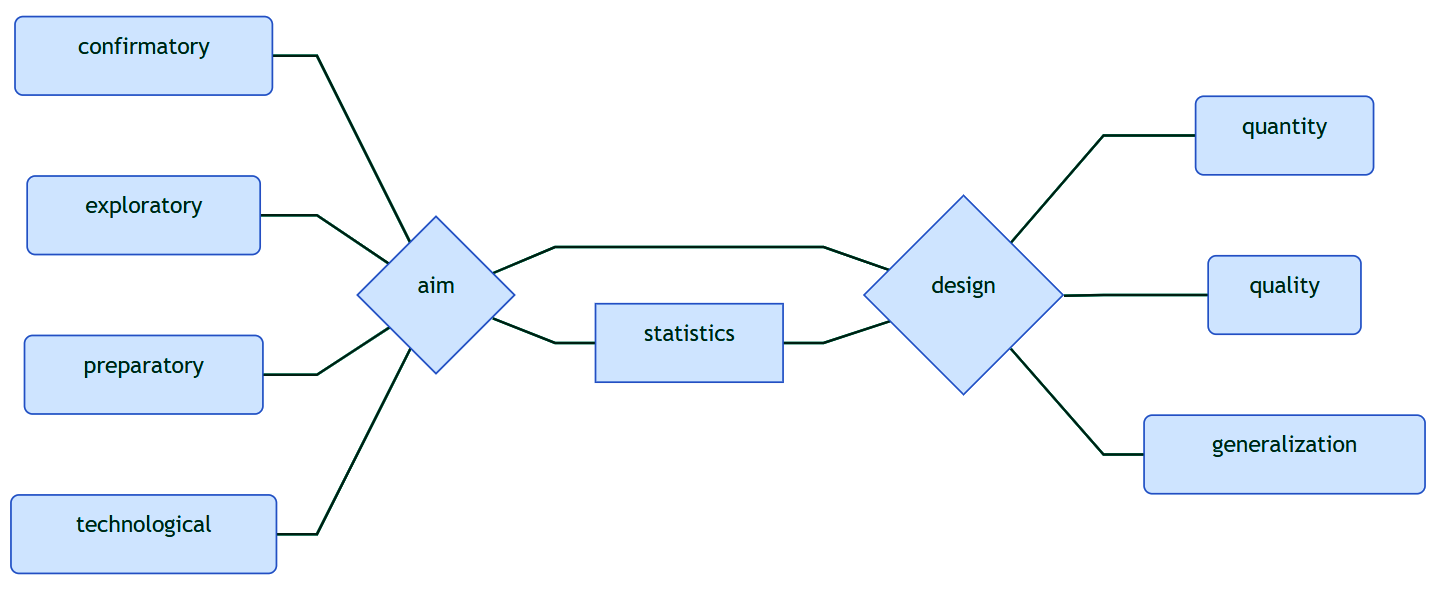
\includegraphics{diagrammeR.png}
\caption{outline: key ingredients and main components}
\end{figure}

\newpage

\subsection{Research Aim}\label{research-aim}

\begin{itemize}
\tightlist
\item
  research aim: concisely express what the study intends to realize

  \begin{itemize}
  \tightlist
  \item
    be specific, if necessary operationalize more general research
    questions explicitly
  \item
    formulate the aim so that it can be evaluated empirically \\
  \end{itemize}
\item
  focus, highlight research questions of primary interest (what at a
  minimum makes your study worthwhile)
\item
  be explicit, for research questions of primary interest specify what
  the results should be -at a minimum- for a successful study
\item
  comment on additional gains the study could offer \\
\item
  example: The aim is to show that the new treatment P is not worse than
  the common treatment Q. The study is successful when the scores on
  measurement Y are maximally 10\% less for P. It will further be
  explored to what extent patient characteristics X could explain the
  scores Y in both treatments.
\end{itemize}

\subsubsection{Categorizations of Research
Aims}\label{categorizations-of-research-aims}

\begin{itemize}
\tightlist
\item
  various categorizations can be considered, for example:

  \begin{itemize}
  \tightlist
  \item
    confirmatory / exploratory / preparatory / technological
  \item
    quantitative / qualitative
  \item
    inferential / descriptive \\
  \end{itemize}
\item
  each type has its properties and requirements
\item
  note: presented type labels are informal, to be used for guidance only
\item
  example: The aim is confirmatory (establish non-inferiority),
  quantitative and inferential (generalization to population).
\end{itemize}

\subsubsection{Confirmatory (purpose A)}\label{confirmatory-purpose-a}

\begin{itemize}
\tightlist
\item
  goal:: confirm an expected difference, relation, \ldots{} maybe the
  aim is to establish a difference or a pre-specified certainty on a
  parameter estimate
\item
  justification based partially on statistical test or accurate
  parameter estimate
\item
  requirement::

  \begin{itemize}
  \tightlist
  \item
    justify what the results -at a minimum- should be (interesting
    enough) referring to significance or accuracy
  \item
    calculate sample sizes to ensure the success of the study (power /
    accuracy of estimation)
  \item
    justify costs and availability of observations implied by required
    sample size
  \item
    explain (statistical) link research design and (especially) primary
    aim 
  \end{itemize}
\item
  note on statistical testing: the aim typically is to show a difference
  (reject equality) but sometimes involves

  \begin{itemize}
  \tightlist
  \item
    non-inferiority/superiority, show conditions are not worse/better
    with a pre-specified margin
  \item
    non-equivalence, show similarity allowing a margin of tolerance
  \item
    absence of evidence is not evidence of absence (only null hypotheses
    can be rejected)
  \end{itemize}
\end{itemize}

\subsubsection{Exploratory (purpose B)}\label{exploratory-purpose-b}

\begin{itemize}
\tightlist
\item
  goal:: explore, evaluate differences, relations, \ldots{} without any
  guarantee on what will be the results
\item
  justification without referring to significance or accuracy

  \begin{itemize}
  \tightlist
  \item
    focus A:: interest in the data as such, descriptive, with results
    being interesting whatever they are

    \begin{itemize}
    \tightlist
    \item
      while testing/accuracy is not the primary aim, it could be
      secondary (significance/accuracy is not guaranteed in advance)
    \end{itemize}
  \item
    focus B:: interest in parameter estimates, with large amounts of
    data available

    \begin{itemize}
    \tightlist
    \item
      without (strong) costs of data collection, or simply because
      available, relations/differences can be evaluated
    \end{itemize}
  \item
    focus C:: interest in evaluations outside the scope of statistical
    testing or estimation

    \begin{itemize}
    \tightlist
    \item
      for example: predictive modeling is evaluated using
      cross-validation (does not include standard errors)
    \end{itemize}
  \item
    focus D:: most qualitative understanding is exploratory
  \end{itemize}
\item
  requirement::

  \begin{itemize}
  \tightlist
  \item
    argument based on substantive grounds or availability/low cost of
    observation
  \item
    explain (statistical) link research design and potential inferences
  \item
    sample size -justification- stresses a balance between information
    and cost
  \end{itemize}
\end{itemize}

\subsubsection{Preparatory (purpose C)}\label{preparatory-purpose-c}

\begin{itemize}
\tightlist
\item
  goal:: prepare for a future study\ldots{} typically a small scale
  set-up
\item
  justification by information offered for future study and merit of
  future study, results are not by themselves of interest

  \begin{itemize}
  \tightlist
  \item
    focus A: phase I and II clinical designs

    \begin{itemize}
    \tightlist
    \item
      decide on whether further studies would be of high enough
      potential while accounting for the costs involved, it requires
      decision criteria to proceed or not
    \end{itemize}
  \item
    focus B: pilot study, which serve to prepare to implement a future
    study

    \begin{itemize}
    \tightlist
    \item
      no statistical testing is implied, that is for the actual study
    \item
      not in itself of interest, therefore not intended for publication
    \item
      could be (partially) qualitative, descriptive, \ldots{} as long as
      it is of interest for the future study
    \end{itemize}
  \item
    focus C: database development or data collection procedures

    \begin{itemize}
    \tightlist
    \item
      no statistical testing is implied, that is for future studies
    \item
      not for publication
    \end{itemize}
  \end{itemize}
\item
  requirement::

  \begin{itemize}
  \tightlist
  \item
    argument based on the information that is still unavailable to set
    up a future study
  \item
    explain how study offers the required but unavailable information
  \item
    sample size -justification- based on an absolute minimal cost

    \begin{itemize}
    \tightlist
    \item
      for example, with animal experiments typically 3 animals per
      condition to allow the estimation of variance
    \end{itemize}
  \end{itemize}
\end{itemize}

\subsubsection{Techn(olog)ical advancements (purpose
D)}\label{technological-advancements-purpose-d}

\begin{itemize}
\tightlist
\item
  goal:: to design, engineer, create, \ldots{} not to extract
  information from the outside world
\item
  justification by the merit of the final product, rarely there is any
  statistics involved
\item
  requirement::

  \begin{itemize}
  \tightlist
  \item
    argument based on what the advancement offers, in balance with the
    costs
  \item
    no statistical justification
  \end{itemize}
\end{itemize}

\subsubsection{Additional distinctions in
aim}\label{additional-distinctions-in-aim}

\begin{itemize}
\tightlist
\item
  quantitative versus qualitative research

  \begin{itemize}
  \tightlist
  \item
    quantitative research focuses on quantifiable empirical aspects

    \begin{itemize}
    \tightlist
    \item
      typically makes use of visualization and statistics to summarize
      and generalize, can be descriptive and/or inferential
    \item
      typically aims to reduce complexity (operationalization before
      data analysis)
    \end{itemize}
  \item
    qualitative research focuses on understanding

    \begin{itemize}
    \tightlist
    \item
      especially focused on reasons, opinions, motivations, \ldots{} ,
      is descriptive and can be hypothesis generating
    \item
      typically embraces complexity 
    \end{itemize}
  \end{itemize}
\item
  descriptive versus inferential research

  \begin{itemize}
  \tightlist
  \item
    inferential, study population using a sample, implies generalization
    and therefore (ideally) representative samples, large enough,
    randomly sampled
  \item
    descriptive, study observed data as such, present data as is without
    reference to uncertainty nor p-values 
  \end{itemize}
\item
  note:: while used here to show distinctions, they can be combined into
  one study
\end{itemize}

\newpage

\subsection{Research Design}\label{research-design}

\begin{itemize}
\tightlist
\item
  the research design is the strategy to achieve the research aim

  \begin{itemize}
  \tightlist
  \item
    it can include data collection, measurement characteristics, and
    even the intended analyses
  \item
    in a strict sense, determines how (potential) observations provide
    information \\
  \end{itemize}
\item
  popular saying: garbage in\ldots{} garbage out !

  \begin{itemize}
  \tightlist
  \item
    a poor design makes a study inefficient at best, completely invalid
    at worst
  \item
    statistics can not solve design problems\\
  \end{itemize}
\item
  there are three types of design attributes, four if you count
  statistics

  \begin{itemize}
  \tightlist
  \item
    quantity of observations (sample size) which should be sufficient
  \item
    quality of observations, dependent on

    \begin{itemize}
    \tightlist
    \item
      conditions under which observations are made
    \item
      what is observed
    \item
      method of observation (how)
    \end{itemize}
  \item
    generalizability (from sample to population), dependent on

    \begin{itemize}
    \tightlist
    \item
      selection of research units
    \item
      missing data mechanism
    \end{itemize}
  \item
    relation with statistical analysis
  \end{itemize}
\end{itemize}

\subsubsection{Quantity of Observations}\label{quantity-of-observations}

\begin{itemize}
\tightlist
\item
  observations should provide information on the questions of interest

  \begin{itemize}
  \tightlist
  \item
    implies more observations are more informative
  \item
    but, observations imply a cost which can be a reason not to make too
    many
  \item
    costs can exist in terms of time, money, risk, stress, \ldots{} 
  \end{itemize}
\item
  justify quantity of observations

  \begin{itemize}
  \tightlist
  \item
    for confirmatory research this includes a sample size -calculation-

    \begin{itemize}
    \tightlist
    \item
      specify statistical test or estimation in focus (should reflect
      what the result -at a minimum- should be to make the study
      successful.
    \item
      specify effect size aimed for, justify both the effect and the
      uncertainty

      \begin{itemize}
      \tightlist
      \item
        effect: what you want to find, ideally justified substantively
        or at least referring to common practice / earlier research
      \item
        uncertainty: variance of your measurement, ideally based on
        earlier data/research or a pilot study
      \item
        use rules of thumb when all reasoning fails, only
      \end{itemize}
    \item
      specify operational characteristics (type I error \(\alpha\) and
      type II error \(\beta\) are related)

      \begin{itemize}
      \tightlist
      \item
        note: an \(\alpha\) of .05 and power of .8 (\(\beta\) = .2)
        imply that type I errors are 4 times more sever than type II
        errors
      \end{itemize}
    \item
      note: do not calculate power / sample size -after- analyzing the
      data
    \end{itemize}
  \item
    typically only required for the primary research questions
  \item
    for exploratory research this includes a sample size -justification-

    \begin{itemize}
    \tightlist
    \item
      feasibility and/or low cost
    \end{itemize}
  \end{itemize}
\end{itemize}

\subsubsection{Quality of Observations}\label{quality-of-observations}

\begin{itemize}
\tightlist
\item
  observations should provide information on the questions of interest

  \begin{itemize}
  \tightlist
  \item
    implies high enough quality which depends on the conditions under
    which observation are made, the method of observation, and what is
    observed
  \item
    with effectiveness (question can be answered) and efficiency (with
    minimal costs) 
  \end{itemize}
\item
  general principle: isolate the effect, either by avoiding or by
  measuring any unwanted influences

  \begin{itemize}
  \tightlist
  \item
    control confounding variables (influence not in the model)
  \item
    maximize systematic variability (explained variance)
  \item
    minimize non-systematic variability (unexplained variance) \\
  \end{itemize}
\item
  note: enforcing general principle typically implies control, at least
  to some extent, over data collection process

  \begin{itemize}
  \tightlist
  \item
    an experimental study exerts control, by definition, thus
    potentially offers higher quality

    \begin{itemize}
    \tightlist
    \item
      necessary condition for causal conclusions
    \end{itemize}
  \item
    observational study does not exert control, efficiency will probably
    reduce

    \begin{itemize}
    \tightlist
    \item
      maybe increase quantity to compensate part of the loss in quality
    \item
      includes naturalistic data collections, surveys, retrospective
      data collection, \ldots{}
    \end{itemize}
  \end{itemize}
\end{itemize}

\subsubsection{Quality of Observations ---
Confounders}\label{quality-of-observations-confounders}

\begin{itemize}
\tightlist
\item
  explain how confounding is avoided

  \begin{itemize}
  \tightlist
  \item
    randomization (large enough sample size), to balance out different
    sources of unwanted influence
  \item
    repeated measures, to keep various sources stable and estimate their
    variance
  \item
    blocking, to keep various sources stable and estimate their variance
  \item
    cross-over designs, to create within unit comparisons and estimate
    order effects
  \item
    matching, to avoid unnecessary unwanted influence
  \item
    (double-) blinding, to avoid unwanted influence from knowing the
    goal of the study
  \item
    and more \ldots{} 
  \end{itemize}
\item
  often more complex designs are more efficient but also more complex to
  analyze (eg., mixed models to deal with repeated measures)
\end{itemize}

\subsubsection{Quality of Observations --- (Non-) Systematic
Variability}\label{quality-of-observations-non--systematic-variability}

\begin{itemize}
\tightlist
\item
  explain how systematic variability is maximized (about including
  everything of importance)

  \begin{itemize}
  \tightlist
  \item
    about the use of proper and well registered explanatory variables
  \item
    about specifying appropriate relations between these variables and
    the observations
  \item
    about the use of maximally differentiating conditions (eg., DOE,
    design of experiments)

    \begin{itemize}
    \tightlist
    \item
      beware: a focus on extremes can introduce artifacts or miss
      important information \\
    \end{itemize}
  \end{itemize}
\item
  explain how non-systematic variability is minimized (about avoiding
  everything irrelevant)

  \begin{itemize}
  \tightlist
  \item
    about the maximization of systematic variability (reduce residual
    error)
  \item
    about the use of proper measurement tools

    \begin{itemize}
    \tightlist
    \item
      ensure reliability / precision to avoid noisy measurements
    \item
      combine measurement tools to estimate reliability
    \end{itemize}
  \item
    about the use of all information available

    \begin{itemize}
    \tightlist
    \item
      avoid the use of categories when continuous registrations are
      available
    \item
      consider multiple imputation when missingness is modest
    \end{itemize}
  \end{itemize}
\end{itemize}

\subsubsection{Generalizability}\label{generalizability}

\begin{itemize}
\tightlist
\item
  explain generalizability (inference)

  \begin{itemize}
  \tightlist
  \item
    about the type of sampling

    \begin{itemize}
    \tightlist
    \item
      probabilistic (sampling: random, stratified, multi-stage,
      \ldots{}.), necessary for conclusive, unbiased, objective
      inferences
    \item
      non-probabilistic (sampling: diversity, expert, \ldots{}.),
      potentially biasing, more subjective, and best used only
      exploratory
    \end{itemize}
  \item
    about missing data

    \begin{itemize}
    \tightlist
    \item
      depends on mechanism of missingness (problem if not at random)
    \item
      explain how it is avoided and dealt with
    \end{itemize}
  \end{itemize}
\end{itemize}

\subsubsection{Small Example}\label{small-example}

The aim is to show that the proposed treatment is an improvement over
the current standard method.

Participants are randomized into two groups, treatment and control. The
control group is given a dummy treatment. A post experiment survey
addresses whether participants were aware about dummy treatment. Each
participant is measured once, immediately after the (dummy) treatment
was administered which results in one score per patient, continuous on a
0-10 scale. A t-test for independent means is used to evaluate whether
the scores in the treatment group are higher than those in the control
group.

A sample size was derived for the t-test to detect a minimal difference
of 2 in favor of the treatment, which was decided upon by our expert
panel. In literature, the standard method is indicated to have a
population standard deviation of about 4. Because no information is
available on the new treatment it is assumed that the same population
standard deviation applies. This leads to a sample size of 51 patients
in each of both groups, required for a one-sided test, type I error of
.05 and power of .8. Earlier experiments showed a drop-out of about
10\%, so 51/9*10 \textless{} 57 patients are included per group.

\newpage

\subsection{Statistics}\label{statistics}

\begin{itemize}
\tightlist
\item
  link between research design and research aim (extra information from
  observations)

  \begin{itemize}
  \tightlist
  \item
    highlight how given a design, statistics is able to resolve the aims

    \begin{itemize}
    \tightlist
    \item
      focus on primary research questions
    \item
      sketch of secondary research questions
    \end{itemize}
  \item
    reflect on the type of data and challenges they offer

    \begin{itemize}
    \tightlist
    \item
      continuous/ordinal/nominal
    \item
      skewed, outliers, boundary values, \ldots{} 
    \end{itemize}
  \end{itemize}
\item
  includes

  \begin{itemize}
  \tightlist
  \item
    statistical tests (evaluate whether effects exist; p-values)
  \item
    statistical estimation (evaluate confidence interval)
  \item
    prediction (evaluate model fit using individual observations)
  \end{itemize}
\item
  introduce intended statistical analysis 
\item
  note: sample size calculations are not part of statistics
\end{itemize}

\newpage

\subsection{Practical Suggestions}\label{practical-suggestions}

\begin{itemize}
\tightlist
\item
  isolate methodological / statistical arguments from substantive
  reasoning
\item
  use consistent labeling of data and conditions
\item
  visualize wherever possible

  \begin{itemize}
  \tightlist
  \item
    data collection process (time-line)
  \item
    categories of observations and their relation
  \item
    design: tables to list conditions between (rows) and within
    (columns)
  \end{itemize}
\end{itemize}

\begin{figure}[htbp]
\centering
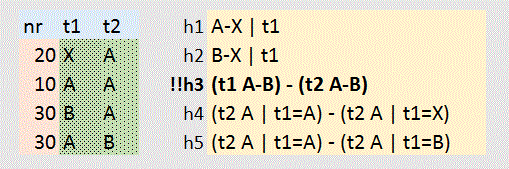
\includegraphics{conds.png}
\caption{example for specifying conditions}
\end{figure}

\subsection{Conclusion}\label{conclusion}

\begin{itemize}
\tightlist
\item
  be clear on your aim and how to reach it with an appropriate design
\item
  be clear on all relevant methodological and statistical aspects of
  your study
\item
  use a language understood by the relevant referee

  \begin{itemize}
  \tightlist
  \item
    statistical lingo
  \item
    visualization
  \end{itemize}
\item
  for support, maybe turn to ICDS 
\end{itemize}

\begin{figure}[htbp]
\centering
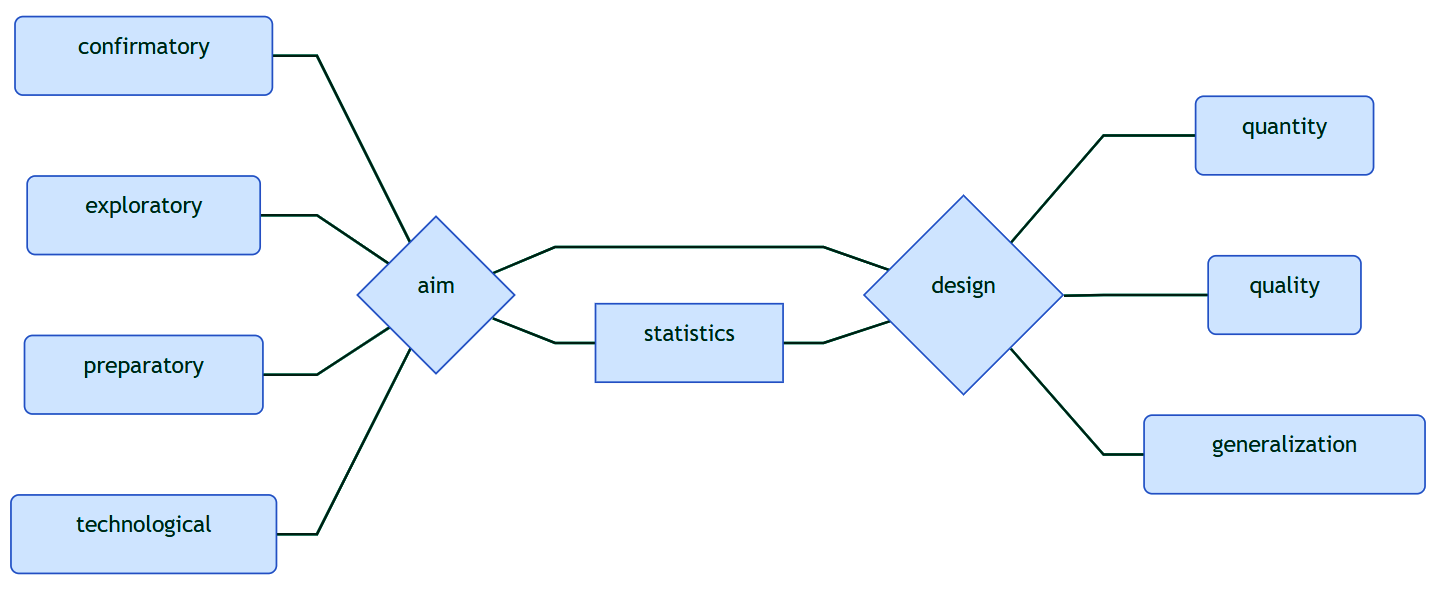
\includegraphics[width=0.70000\textwidth]{diagrammeR.png}
\caption{reminder: key ingredients and main components}
\end{figure}

\newpage

\section{\texorpdfstring{\protect
\includegraphics[width=0.40000\textwidth]{icds.png}}{}}\label{section}

Methodological and statistical support to help make a difference

\begin{itemize}
\item
  ICDS provides complementary support in methodology and statistics to
  our research community, for both individual researchers and research
  groups, in order to get the best out of them
\item
  ICDS aims to address all questions related to quantitative research,
  and to further enhance the quality of both the research and how it is
  communicated
\end{itemize}

website: \url{https://www.icds.be/} includes information on who we
serve, and how

booking: \url{https://www.icds.be/consulting/} for individual
consultations

\end{document}
